\documentclass[a4paper,11pt]{report}

\usepackage[T1]{fontenc}
\usepackage[utf8]{inputenc}
\usepackage{xcolor} 
\usepackage{siunitx}
\usepackage[version=4]{mhchem}
\usepackage{booktabs}
\usepackage{graphicx}
\usepackage{amsmath}
\usepackage{circuitikz}
\usepackage{fancyhdr}
\usepackage{titlesec}
\usepackage{totpages}
\usepackage{transparent}
\usepackage{tikz}
\usepackage{helvet}
\usepackage{pdfpages}
\usepackage[margin=2.5cm, headheight=1.4cm]{geometry}
\graphicspath{{image/}}

%Site pour forme : https://tikzmaker.com/editor

% Définitions espace avant chapitre
\titleformat{\chapter}[hang]{\normalfont\huge\bfseries}{\thechapter}{20pt}{\Huge}
\titlespacing*{\chapter}{0pt}{0pt}{15pt}

% Définition du texte atténué
\newcommand{\faintText}[1]{\textcolor{black!35}{\small #1}}
\definecolor{insared}{RGB}{220, 20, 30}
\definecolor{titlegray}{RGB}{145, 150, 155}
\definecolor{authorgray}{RGB}{125, 130, 135}

% Configuration globale de fancyhdr
\pagestyle{fancy}
\fancyhf{}

% Haut de page
\fancyhead[L]{$\vcenter{\hbox{\faintText{\leftmark}}}$}
\fancyhead[C]{$\vcenter{\hbox{\faintText{S-IoT - Project Report : Drone swarm}}}$}
\fancyhead[R]{$\vcenter{\hbox{\transparent{0.5}
\includegraphics[height=1.2cm]{Logo INSA.png}}}$}
\renewcommand{\headrulewidth}{0.4pt}
\renewcommand{\headrule}{\hbox to\headwidth{\color{black!20}\leaders\hrule height \headrulewidth\hfill}}

% Bas de page
\fancyfoot[C]{\faintText{Page \thepage\ on \ref{TotPages}}}
\renewcommand{\footrulewidth}{0pt}

\fancypagestyle{plain}{
    \fancyhf{}
    \fancyhead[L]{$\vcenter{\hbox{\faintText{\leftmark}}}$}
    \fancyhead[C]{$\vcenter{\hbox{\faintText{S-IoT - Project Report : Drone swarm}}}$}
    \fancyhead[R]{$\vcenter{\hbox{\transparent{0.5}
\includegraphics[height=1.2cm]{Logo INSA.png}}}$}
    \fancyfoot[C]{\faintText{Page \thepage\ on \ref{TotPages}}}
    \renewcommand{\headrulewidth}{0.4pt}
    \renewcommand{\headrule}{\hbox to\headwidth{\color{black!20}\leaders\hrule height \headrulewidth\hfill}}
}

\begin{document}
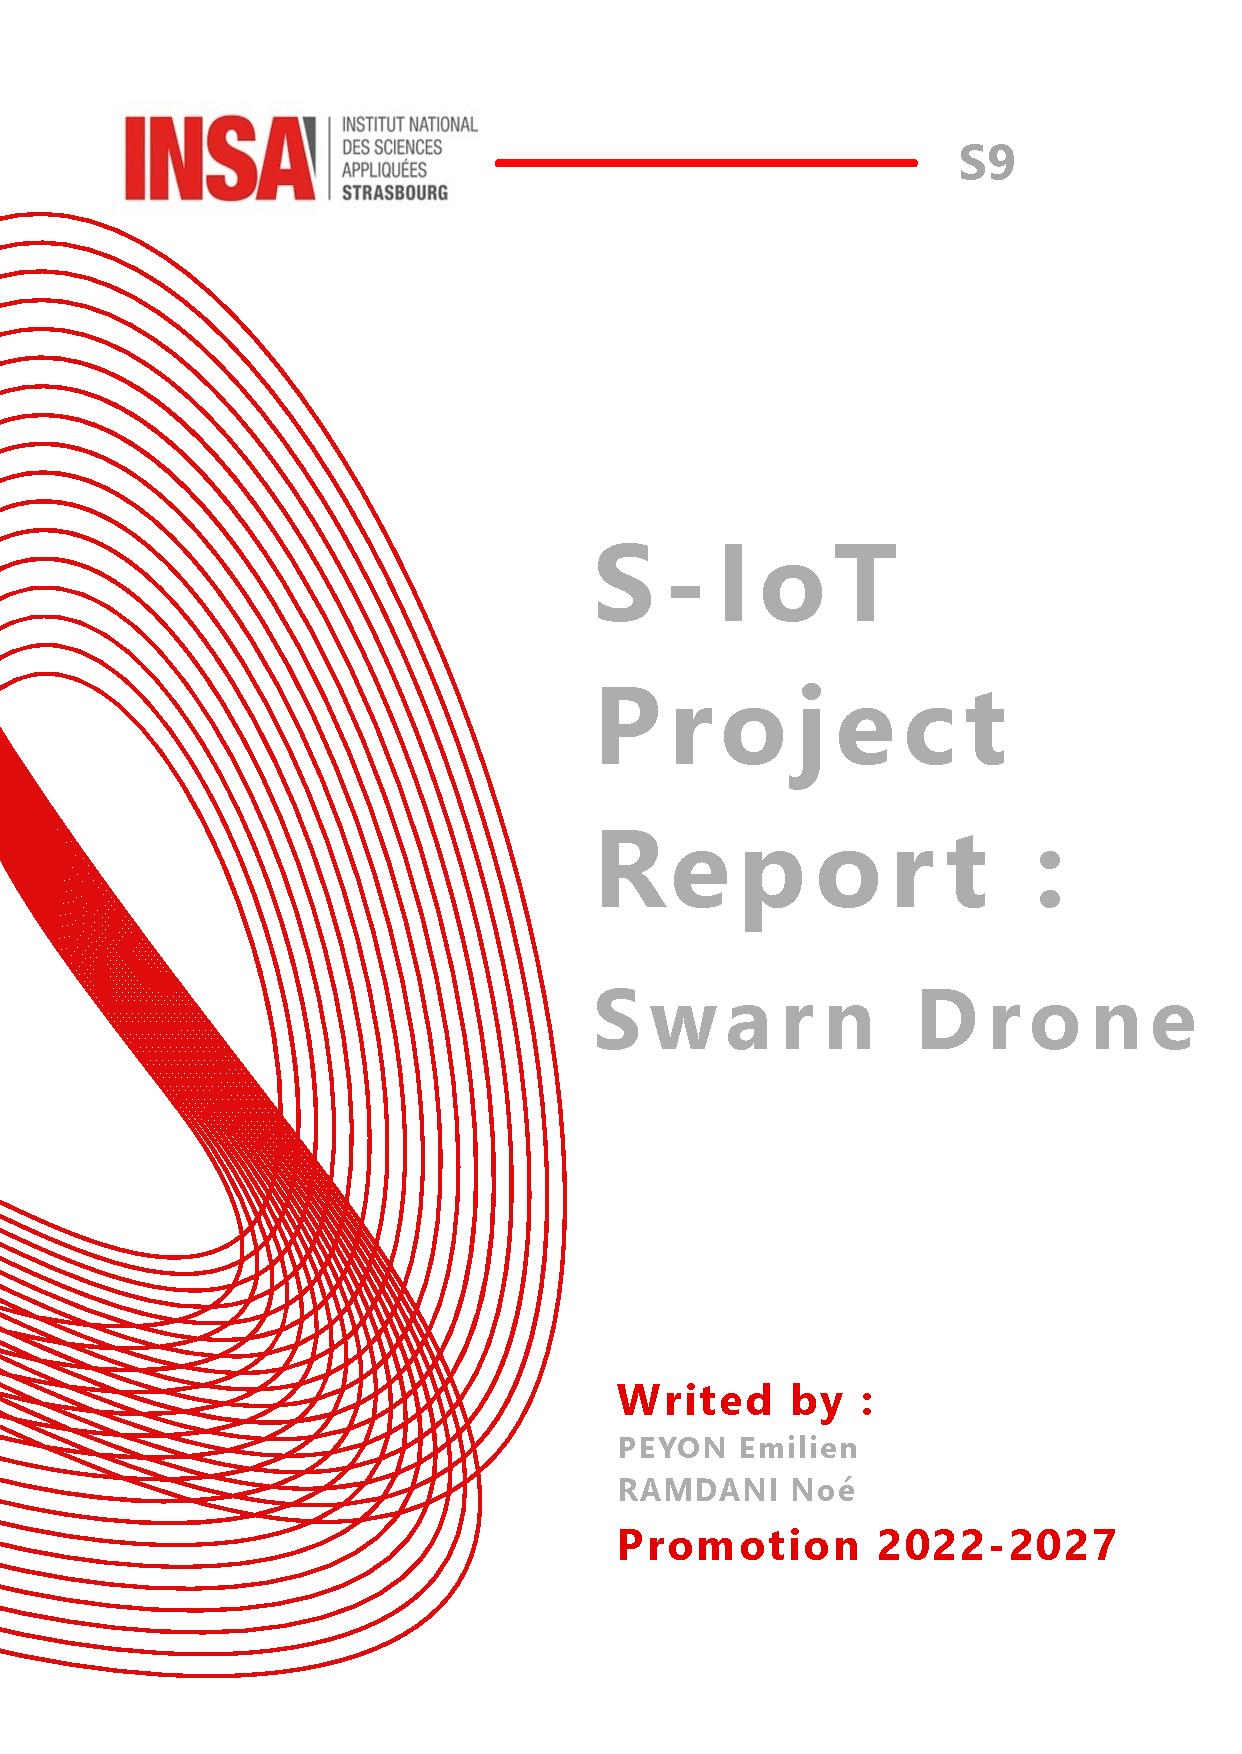
\includepdf[pages=1]{PrePage/PageDeGarde.pdf}
\newpage
\chapter*{Specifications}
\markboth{Specifications}{Specifications}

\section*{Objective}
The purpose of this project is to fly a swarm of UAVs (2 to 3 UAVs) and try to lift off a payload using a net.
\section*{Functions}
\begin{itemize}

    \item UWB precise location system
    \item PID Controller for drone stabilization 
    \item UWB Communication for high frequency refreshing data
    \item Make a simple back and forth keeping the drone formation (following a leader ?)

\end{itemize}

\section*{Deliverable}
\begin{itemize}

    \item Report with all progress, advancements and explanation of technical knowledge
    \item Functional UWB code 
    \item Methodology and results of calibration of UWB sensors
    \item Bibliographical Studies
    \item Video of Drone demo 
    \item Functional PID Corrector
    \item Functional ESP32 code implementation using Multi-threading

\end{itemize}



\newpage
\chapter*{Bibliographical Studies}
\markboth{Bibliographical Studies}{Bibliographical Studies}

\section{UWB}

\subsection{Definitions}
Explain what is UWB
\subsection{Algorithm}
Explain that we found and test different Algorithm
\subsubsection{Two way ranging (TWR)}
The Two Way Ranging (TWR) algorithm is the easiest and the fastest to implement in a UWB system.
In order to explain this algorithm,  we will use 2 modules called $UWB_1$ and $UWB_2$.

\begin{figure}[!ht]
\centering
\resizebox{0.7\textwidth}{!}{%
\begin{circuitikz}
\tikzstyle{every node}=[font=\fontsize{18.2pt}{23.7pt}\selectfont]
\draw  (5,9) circle (1.25cm);
\draw  (15,9) circle (1.25cm);
\draw [-{Stealth[scale=1.5]}, ] (6.25,10.25) -- (13.75,10.25);
\draw [-{Stealth[scale=1.5]}, ] (13.75,7.75) -- (6.25,7.75);
\node [font=\fontsize{18.2pt}{23.7pt}\selectfont, inner xsep=0.080cm, inner ysep=0.085cm, rounded corners=0.020cm] at (14.875,9) {UWB};
\node [font=\fontsize{18.2pt}{23.7pt}\selectfont, inner xsep=0.080cm, inner ysep=0.085cm, rounded corners=0.020cm] at (4.875,9) {UWB};
\node [font=\fontsize{18.2pt}{23.7pt}\selectfont, inner xsep=0.080cm, inner ysep=0.085cm, rounded corners=0.020cm] at (10,10.75) {POLL};
\node [font=\fontsize{15.9pt}{20.7pt}\selectfont, inner xsep=0.080cm, inner ysep=0.085cm, rounded corners=0.020cm] at (5.75,8.875) {1};
\node [font=\fontsize{15.9pt}{20.7pt}\selectfont, inner xsep=0.080cm, inner ysep=0.085cm, rounded corners=0.020cm] at (15.75,8.875) {2};
\node [font=\fontsize{18.2pt}{23.7pt}\selectfont, inner xsep=0.080cm, inner ysep=0.085cm, rounded corners=0.020cm] at (10,7.25) {RESP};
\node [font=\fontsize{18.2pt}{23.7pt}\selectfont, inner xsep=0.080cm, inner ysep=0.085cm, rounded corners=0.020cm] at (6.125,10.875) {$t_{x1}$};
\node [font=\fontsize{18.2pt}{23.7pt}\selectfont, inner xsep=0.080cm, inner ysep=0.085cm, rounded corners=0.020cm] at (6.125,7.25) {$r_{x1}$};
\node [font=\fontsize{18.2pt}{23.7pt}\selectfont, inner xsep=0.080cm, inner ysep=0.085cm, rounded corners=0.020cm] at (13.875,10.875) {$r_{x2}$};
\node [font=\fontsize{18.2pt}{23.7pt}\selectfont, inner xsep=0.080cm, inner ysep=0.085cm, rounded corners=0.020cm] at (13.875,7.25) {$t_{x2}$};
\end{circuitikz}
}%
\caption{TWR explanation diagram}
\label{fig:TWR}
\end{figure}
\noindent The algorithm works in 4 steps :  
\begin{enumerate}
    \item $UWB_1$ send a \textbf{POLL} to $UWB_2$. The time of emission $t_{x1}$ is memorized by $UWB_1$.
    \item $UWB_2$ receive the \textbf{POLL} and memorize the time of arrival $r_{x2}$.
    \item $UWB_2$ process the \textbf{POLL}, and precisely plan the time of emission $t_{x2}$ for the \textbf{RESP}. It contains ($t_{x2},r_{x2}$).
    \item $UWB_1$ receive the \textbf{RESP} and memorize the $r_{x1}$.
\end{enumerate}
With all those parameters, we can deduce those variables :
\begin{itemize}
    \item Total time : $t_{tot} = r_{x1} - t_{x1}$
    \item Processing time of $UWB_2 : t_{proc} = r_{x2} - t_{x2}$
    \item Travel time : $t_{travel} = t_{tot} - t_{proc}$
\end{itemize}
The signal travels back and forth so it did twice the distance ($d$), and travel speed of a radio signal is equivalent to light speed ($c$). \\ 
So, we can deduce this equation : 
\begin{equation} \label{TWR_eq}
\boxed{\frac{t_{travel}\times c}{2}=\frac{(t_{tot} - t_{proc}) \times c}{2}= \frac{((r_{x1} - t_{x1}) - (r_{x2} - t_{x2})) \times c}{2}}
\end{equation}
We can also determine the induced error of this algorithm.\\
After calculation (describe in calculation part at page~\pageref{TWR-Error-calculation}), we obtain this equation: 
\begin{equation}
\epsilon \approx \frac{t_ {proc}(e_a - e_b)}{2}
\end{equation}
As we can observe, the Time of processing is directly link to the error. The $t_{proc}$ is around 3,000,000 nanoseconds so, it's inducing a high error. 
 
\subsubsection{Double Sided Two way ranging (DS-TWR)}
The DS-TWR has for purpose to reduce the error introduce by the $t_{proc}$. This algorithm also use $UWB_1$ and $UWB_2$.

\begin{figure}[!ht]
\centering
\resizebox{0.7\textwidth}{!}{%
\begin{circuitikz}
\tikzstyle{every node}=[font=\fontsize{18.2pt}{23.7pt}\selectfont]
\draw  (5,9) circle (1.25cm);
\draw  (15,9) circle (1.25cm);
\draw [-{Stealth[scale=1.5]}, ] (13.75,7.75) -- (6.25,7.75);
\node [font=\fontsize{18.2pt}{23.7pt}\selectfont, inner xsep=0.080cm, inner ysep=0.085cm, rounded corners=0.020cm] at (14.875,9) {UWB};
\node [font=\fontsize{18.2pt}{23.7pt}\selectfont, inner xsep=0.080cm, inner ysep=0.085cm, rounded corners=0.020cm] at (4.875,9) {UWB};
\node [font=\fontsize{18.2pt}{23.7pt}\selectfont, inner xsep=0.080cm, inner ysep=0.085cm, rounded corners=0.020cm] at (10,9.5) {POLL};
\node [font=\fontsize{15.9pt}{20.7pt}\selectfont, inner xsep=0.080cm, inner ysep=0.085cm, rounded corners=0.020cm] at (5.75,8.875) {1};
\node [font=\fontsize{15.9pt}{20.7pt}\selectfont, inner xsep=0.080cm, inner ysep=0.085cm, rounded corners=0.020cm] at (15.75,8.875) {2};
\node [font=\fontsize{18.2pt}{23.7pt}\selectfont, inner xsep=0.080cm, inner ysep=0.085cm, rounded corners=0.020cm] at (10,7.25) {RESP};
\node [font=\fontsize{18.2pt}{23.7pt}\selectfont, inner xsep=0.080cm, inner ysep=0.085cm, rounded corners=0.020cm] at (6.125,10.875) {$t_{x1}$};
\node [font=\fontsize{18.2pt}{23.7pt}\selectfont, inner xsep=0.080cm, inner ysep=0.085cm, rounded corners=0.020cm] at (6.125,7.25) {$r_{x1}$};
\node [font=\fontsize{18.2pt}{23.7pt}\selectfont, inner xsep=0.080cm, inner ysep=0.085cm, rounded corners=0.020cm] at (13.875,10.875) {$r_{x2}$};
\node [font=\fontsize{18.2pt}{23.7pt}\selectfont, inner xsep=0.080cm, inner ysep=0.085cm, rounded corners=0.020cm] at (13.875,7.25) {$t_{x2}$};
\draw [{Stealth[scale=1.5]}-, ] (13.625,10.125) -- (6.125,10.125);
\draw [{Stealth[scale=1.5]}-, ] (13.5,11.75) -- (6,11.75);
\node [font=\fontsize{18.2pt}{23.7pt}\selectfont, inner xsep=0.080cm, inner ysep=0.085cm, rounded corners=0.020cm] at (9.625,11.25) {FINAL};
\node [font=\fontsize{18.2pt}{23.7pt}\selectfont, inner xsep=0.080cm, inner ysep=0.085cm, rounded corners=0.020cm] at (6.125,12.5) {$t_{x12}$};
\node [font=\fontsize{18.2pt}{23.7pt}\selectfont, inner xsep=0.080cm, inner ysep=0.085cm, rounded corners=0.020cm] at (13.75,12.5) {$r_{x22}$};
\end{circuitikz}
}%
\caption{DS-TWR explanation diagram}
\label{fig:DS-TWR}
\end{figure}

\section{Data treatment}

\subsection{Polynomiale Filter}

\subsection{Filter}

\subsubsection{Kaalman Filter}

\subsubsection{Extended Kaalman Filter}

\newpage
\chapter*{Caculations}
\subsection*{TWR Error calculation : } \label{TWR-Error-calculation}
Let's set: 
\begin{itemize}
\item True time of flight : $T_{f}$
\item True time of process : $t_{proc}$
\item Clock drift errors : $e_a$ and $e_b$
\end{itemize}
The measured times are: 
\begin{equation}
R_a = (2T_f + t_{proc})(1 + e_a) \text{ and } t_{proc_b} = t_{proc}(1 + e_b)
\end{equation}
The calculated time of flight is:
\begin{equation}
\hat{T}_f = \frac{R_a -t_{proc_b}}{2}
\end{equation}
By replacing $R_a$ and $t_{proc_b}$, we obtain : 
\begin{equation}
\hat{T}_f = \frac{2T_f(1 + e_a) + t_{proc}(1 + e_a) - t_{proc}(1 + e_b)}{2}
\end{equation}
By simplifying, we obtain :
\begin{equation}
\hat{T}_f = T_f(1 + e_a) + \frac{t_{proc}(e_a - e_b)}{2}
\end{equation}
The error is $\hat{T}_f - T_f$, so: \\
\begin{equation}
Error = T_f \times e_a + \frac{t_{proc}(e_a - e_b)}{2}
\end{equation}
The time of flight is about 33 nanoseconds, however D is around $3,000,000$. \\
So we can ignore $T_f \times e_a$ cause $T_{f} \ll t_{proc}$, and we obtain :
\begin{equation}
Error \approx \frac{t_{proc}(e_a - e_b)}{2}
\end{equation}
\subsection*{DS-TWR Error calculation : } \label{DS-TWR-Error-calculation}

\end{document}